% !TeX root = main.tex
\chapter{Introduction}
To survive in an ecosystem organisms need to adapt to the specific abiotic and biotic factors around them. This is particularly important for plants since they can not change their habitat during their lifespan. Adaptation can operate on different levels of the organisms from the adaptation of protein function to modifications in cell functions or whole tissue functions. But the underlying fundamental process that drives adaptation is the modification of the genetic material DNA.\\
Modifications on DNA level are called mutations and in four different groups. In the following description we consider just mutations which occur in coding regions of the genome although they can be distributed throughout all regions of the genome. A point mutation, which is the first group of mutations and can be also called single nucleotide polymorphism (SNP), is concerning just one single base pair. These changes the DNA sequence on one single point and therefore lead to changes of the transcribed mRNA. The second class of mutations are insertions. These insert a new sequence into the former DNA sequence and thus elongate it. These insertions can have a variety of length from one single bp to a few hundred bp and even longer sequences can be added.  The contrasting class of insertions are deletions, which lead to a reduction of base pairs in a variety of lengths in the former DNA strand. The last category of mutations are duplications. As implied by the name, regions of the DNA get duplicated and inserted at a different position. The regions can be copied abnormally one or even more times.\\
These mutations are first of all just changes in the DNA but indirectly they impact all the resulting processes. The DNA first gets transcribed into mRNA. This process is not affected by the evolved mutations. But after the transcription the mRNA gets translated into proteins. In this step the impact of the mutations appear since a triplet codon gets translated into a specific amino acid, which can change due to the mutation in the DNA as postulated by Gamow\cite{crick1988}. The mutations can have different effects on the resulting protein. The insertions or deletions lead mostly to a shift in the reading frame and therefore change the sequence of amino acids in a wide range. Point mutations, although they change just a single codon, can have different effects on the translated amino acid and therefore on the functionality of the resulting protein. As it was known that 20 amino acids exists and when the knowledge arises that a codon includes three base pairs the genetic code could get deciphered by \textcite{Nirenberg1965}. The gain of knowledge deciphering this genetic code showed that the genetic code is degenerated as identified by \textcite{Lagerkvist1978}, which means that not one codon is directly linked to an amino acid rather that there are multiple codons that can initiate the same amino acid, which is showed in \autoref{fig:Codons} a). For the topic of point mutations we have three possible outcomes resulting after such mutation. The first outcome is a synonymous mutation, which is the less severe one and does not change the protein at all. Here a base pair changes but the translated codons provoke the same amino acid. An schematic representation of synonymous mutations can be found in \autoref{fig:Codons} b). As shown in \autoref{fig:Codons} c) a mutation could also be a non-synonymous mutation where the modified codon leads to an exchange of the amino acid type. The prediction of how severe these non-synonymous mutations are is hard to do without further analysis. It depends on many circumstances for example if the location is a catalytic region or to which other amino acid it is exchanged. Such a mutation can be very unnoticeable or on the other hand making the protein non-functional. The last kind of point-mutations are premature stop codons. They represent a mutation of a usual codon to a stop codon as it can be seen in \autoref{fig:Codons}d). This means most of the time drastic changes in the protein functionality since the resulting protein is truncated. Thereby premature stop codons represent the most interesting kind of mutations for understanding adaptation in plants since they can be recognized in the DNA level and they should change the function of the truncated protein.\\
\begin{figure}[tb]
    \centering
    \begin{minipage}[h]{0.9\textwidth}
      \centering
      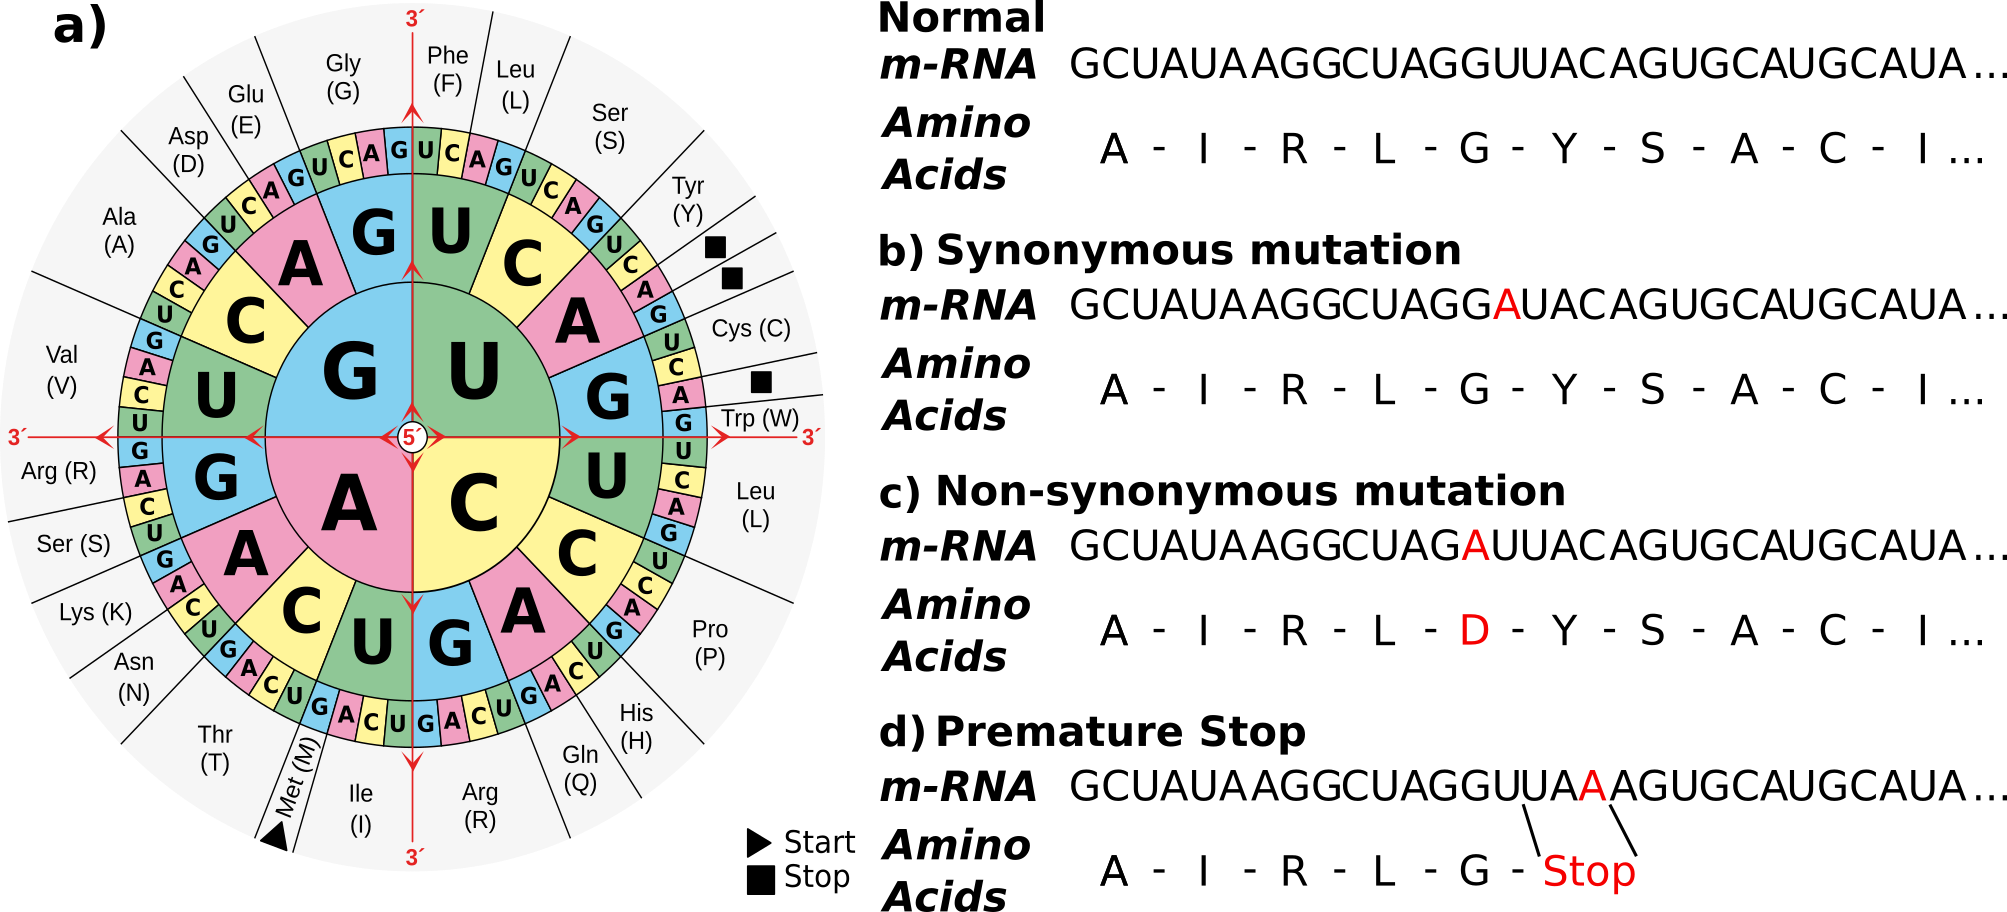
\includegraphics[width=1\textwidth]{images/Mutations.png}
      \caption{\textbf{Schematic representation of point mutation classes}\\
      a) The genetic code (image taken from \textcite{bresch2013}); b) A schematic representation of a synonymous mutation, which affects the mRNA but not the amino acid sequence. c) A schematic representation of a non-synonymous mutation. The change of a single base pair in the mRNA sequence changes to an exchange of the amino acid type. d) A schematic representation of a premature stop codon. Retrieved from a exchange of a single base pair an premature stop codon appears and stops the amino acid sequence.}
     \label{fig:Codons}
    \end{minipage}
  \end{figure}
Until recently in evolutionary theories the axiom exists that these described mutations occur randomly throughout the genome and that solely after occurrence of mutations the evolutionary selection operates and shapes the genetic pool of a population\cite{futuyma1986}. From this axiom it can be deduced that natural selection acts on this mutations by classifying fatal modifications and filter these out of the genetic pool. The time span during which this genetic pool adapts to a single mutation is depending on the severity of the modification. That also implies that mutations which have a neutral significance like synonymous mutations are not shaped by the selection force. On the other side positive impact is reinforced by the selection force so that these mutations get accumulated in the genetic pool\cite{darwin1909}.\\
If one now only considers the mutation type premature stop codons some hypotheses can be used to explain the effects of mutations on gene regulatory networks. Since the occurence of premature stop codons is leading directly to a loss of function in this protein one can consider that the evolutionary selection force stabilizes the gene regulatory networks by maintaining the diversion of this networks. Practically this means that if a protein is knocked out by a premature stop codons the pathways around this gene are getting more important and you expect that they are under a high conservation force by evolutionary selection and selection prevent a accumulation of premature stop codons in the rest of the gene regulatory network.\\
In our following project we want to study the attributes and occurence of these premature stop codons. We want to characterize how the natural selection is shaping population structures through generating loss-of-function variants and how they affect the adaptation process of organisms. We therefore follow a bioinformatical approach by applying data analysis and statistical algorithms on different genomic data and with these try to find evolutionary patterns. 